\chapter{Studying Instrinsic Channel Properties, Scattering Mechanisms, and Quantum Transport}\label{chap:results}
Developing low resistance two-dimensional/two-dimensional (2D/2D) ohmic contacts opens up possibility to study the intrinsic properties of \acp{TMD} and quantum physics. In particular, quantum phenomena inherent to \acp{2DEG} and \acp{2DHG} such as the integers and fractional quantum Hall effects and \ac{SdH} oscillations can be explored in high mobility monolayer and few-layer \acp{TMD} \cite{Cui_NatureNano2015}. In addition to quantum transport properties and quantum effects in monolayer and few-layer \acp{TMD} the study of mobility and its corresponding temperature dependence can be used to understand the multiple scattering mechanisms present \cite{Kaasbjerg_PhysRevB2012}. These study of both electron and hole transport mechanisms is important due to the fact that high-performance $p$-type and $n$-type transistors are necessary for complimentary digital applications. 

\section{$p$-type \ch{MoS2} Semiconductor Doping}\label{sec:mos2_doping}
One of the major challenges that still remains in fabricating devices to study quantum transport and scattering mechanisms is developing high quality $p$-type \ch{MoS2} devices. This is due to the fact that the metal/\ch{MoS2} interface is obstructed by a large \ac{SB} formed by Fermi level pinning close to the conduction band of the \ch{MoS2} \cite{Chuang_NanoLett2014,Das_NanoLett2012}. 

\subsection{$p$-type \ch{MoS2} and \ch{WSe2} Semiconductor Contact Resistance}\label{subsec:mos2_doping_contact}
To study the effects of doping and how it affects the \ac{SBH} several \ch{MoS2} device geometries were designed. In particular, the purpose is to find how doping \ch{MoS2} and \ch{WSe2} can help improve the 2D/2D contacts in devices and, in addition, how doping the channel affects the intrinsic properties of the device. To address the the issue of contact resistance, transmission devices were designed in which electrodes are spaced at varying lengths from the source electrode. Resistance is given by 
\begin{equation}\label{eq:resistance_fundamental}
R = \frac{\rho}{A} l,
\end{equation}
where, in this case, it is assumed that the resistivity $\rho$ and the area $A$ are constant throughout. Thus the resistance $R$ is then proportional to $l$. By determining the resistance as a function of length one can determine the inherent contact resistance of the device. Fig.~\ref{fig:transmission_NbMoS2_devices} illustrates the design of several $0.05\%$ \ch{WSe2} doped \ch{WSe2} transmission devices with varying lengths of electrodes.
\begin{figure}[ht]
	\centering
	\subfloat[$0.05\%$ \ch{Nb} doped \ch{WSe2} channel transmission device with corresponding channel lengths and widths of $L_{12} = 1.04\unita{\mu m}$ $W_{12} = 4.42\unita{\mu m}$, $L_{23} = 2.04\unita{\mu m}$, $W_{23} = 4.47\unita{\mu m}$, $L_{34} = 3.09\unita{\mu m}$, $W_{34} = 4.90\unita{\mu m}$, $W_{45} = 5.15\unita{\mu m}$, and $L_{45} = 4.27\unita{\mu m}$. ]{
		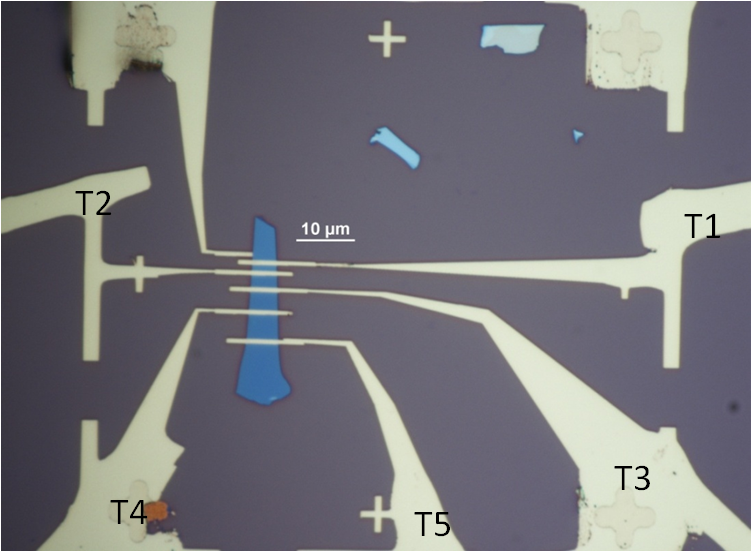
\includegraphics[height=4cm,width=6cm]{figs/results/transmission_device_pic_5-5_21_10232015_no1}
		\label{fig:transmission_device_10232015_no1}
	}
	\qquad
	\subfloat[Caption here]{
		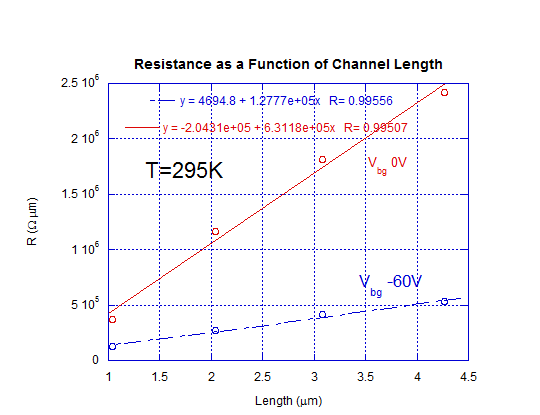
\includegraphics[height=4cm,width=6cm]{figs/results/transmission_resistance_plot_pic_5-5_21_10232015_no1}
		\label{fig:transmission_device_10232015_no1_resistance}
	}

	\subfloat[$0.05\%$ \ch{Nb} doped \ch{WSe2} channel transmission device with corresponding channel lengths and widths of $L_{12} = 0.42\unita{\mu m}$, $W_{12} = 2.27\unita{\mu m}$, $L_{23} = 0.83\unita{\mu m}$, $W_{23} = 2.30\unita{\mu m}$, $L_{34} = 2.01\unita{\mu m}$, $W_{34} = 2.27\unita{\mu m}$, $W_{45} = 2.45\unita{\mu m}$, and $L_{45} = 3.02\unita{\mu m}$.]{
		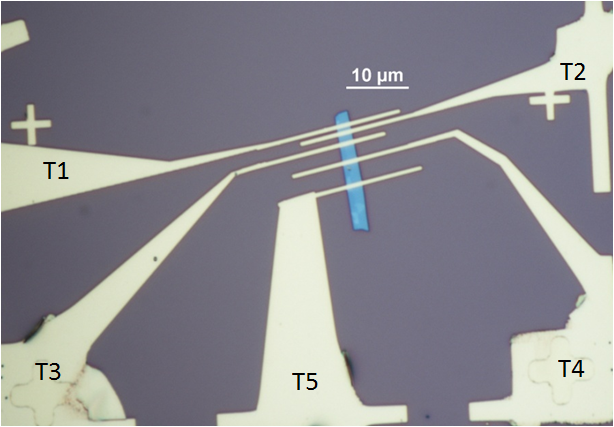
\includegraphics[height=4cm,width=6cm]{figs/results/transmission_device_pic_56_21_10232015_no2}
		\label{fig:transmission_device_10232015_no2}
	}
	\qquad
	\subfloat[Caption here]{
		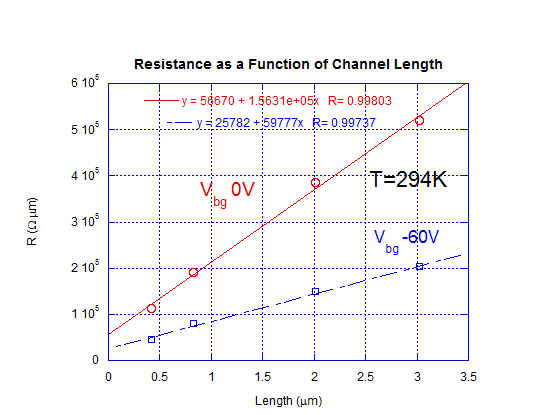
\includegraphics[height=4cm,width=6cm]{figs/results/transmission_resistance_plot_pic_56_21_10232015_no2}
		\label{fig:transmission_device_10232015_no2_resistance}
	}

	\subfloat[$0.05\%$ \ch{Nb} doped \ch{WSe2} channel transmission device with corresponding channel lengths and widths of $L_{12} = 0.43\unita{\mu m}$, $W_{12} = 2.10\unita{\mu m}$, $L_{23} = 0.93\unita{\mu m}$, $W_{23} = 1.90\unita{\mu m}$, $L_{34} = 1.34\unita{\mu m}$, $W_{34} = 1.98\unita{\mu m}$, $L_{56} = 2.00\unita{\mu m}$, $W_{56} = 1.89\unita{\mu m}$, $W_{67} = 1.80\unita{\mu m}$, and $L_{67} = 2.58\unita{\mu m}$.]{
		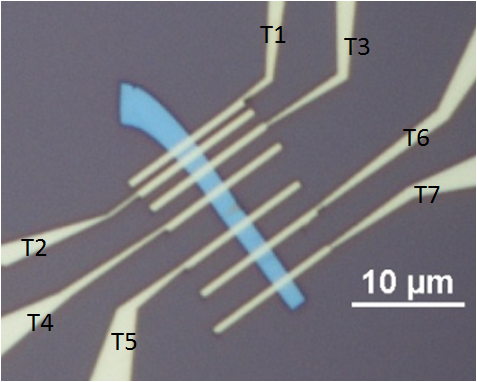
\includegraphics[height=4cm,width=6cm]{figs/results/transmission_device_pic_-66_21_11182015_no2}
		\label{fig:transmission_device_11182015_no2}
	}
	\qquad
	\subfloat[Caption here]{
		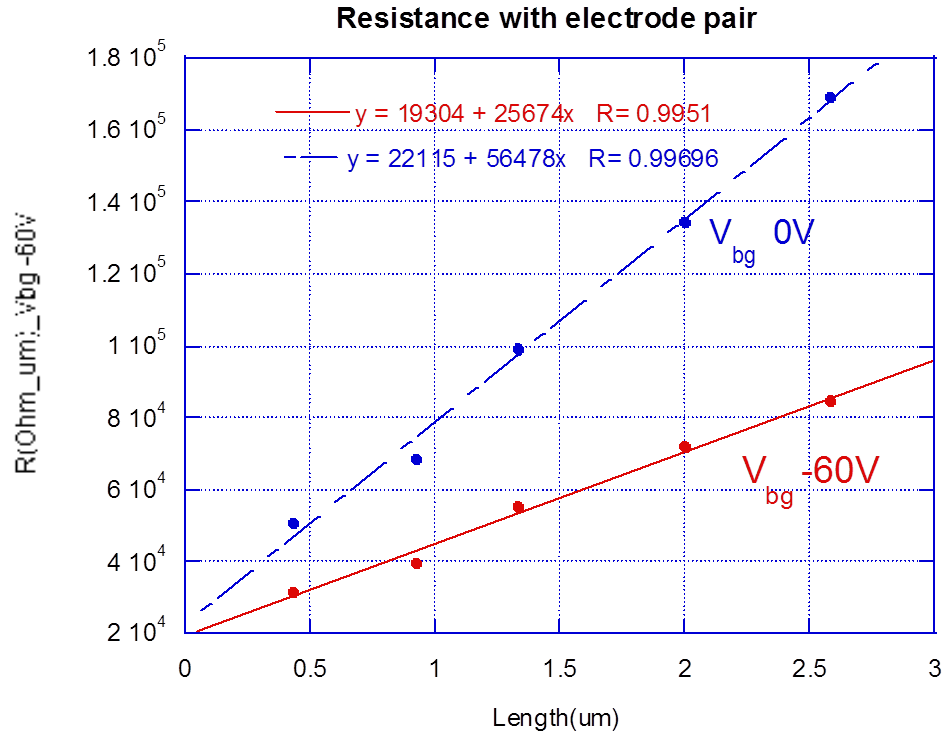
\includegraphics[height=4cm,width=6cm]{figs/results/transmission_resistance_plot_pic_-66_21_11182015_no2}
		\label{fig:transmission_device_11182015_no2_resistance}
	}

	\caption[0.05\% \ch{Nb} doped \ch{WSe2} transmission devices]{Several 0.05\% \ch{Nb} doped \ch{WSe2} transmission devices with varying lengths and widths.}
	\label{fig:transmission_NbMoS2_devices}
\end{figure}

\subsection{$p$-type \ch{MoS2} and \ch{WSe2} Semiconductor Intrinsic Channel Properties}\label{subsec:mos2_intrinsic_properties}
\begin{figure}[ht]
	\centering
	\subfloat[caption here]{
		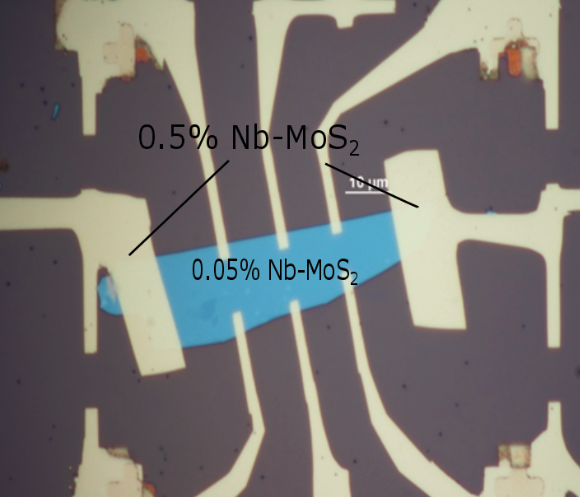
\includegraphics[height=4cm,width=6cm]{figs/results/hall_bar_device_pic_5-5_21_10152015_no2_modified}
		\label{fig:hall_bar_10152015_no2_modified}
	}
	\qquad
	\subfloat[caption here]{
		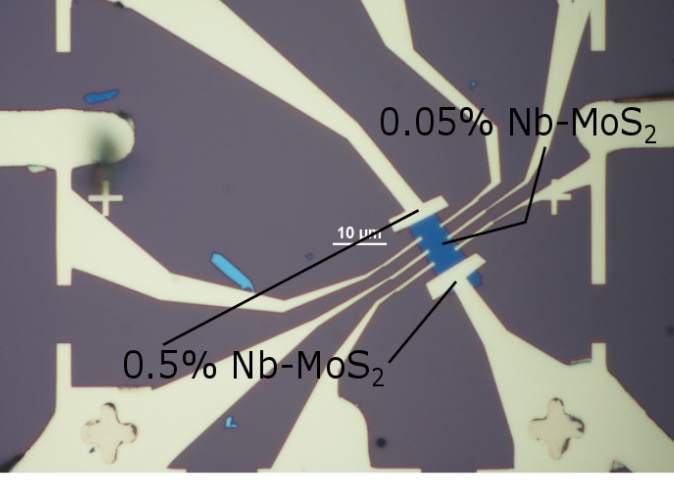
\includegraphics[height=4cm,width=6cm]{figs/results/hall_bar_device_pic_11182015_no2_modified}
		\label{fig:hall_bar_11182015_no2_modified}
	}
	\caption[Hall bar devices]{Caption here}
	\label{fig:hall_bar_NbMoS2_devices}
\end{figure}
 
